'%\begin{ccHtmlOnly}
%<center>
%<img border=0 src="./saarhull.gif" align=middle>
%</center>
%\end{ccHtmlOnly} 
%
%\begin{ccTexOnly}
%\begin{center}
%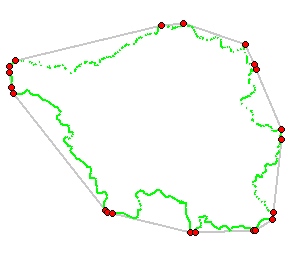
\includegraphics[width=6.5cm]{Convex_hull_2/saarhull}
%%\leavevmode\epsfxsize8cm\epsffile{Convex_hull_2/saarhull.eps}
%\end{center}
%\end{ccTexOnly}

\section{Spatial Sorting\label{sec:spatial_sorting}}

\cgal\ provides a small set of sorting algorithms, currently implemented only for 2D and 3D points, although it is easy to extend them to other objects through a traits mechanism.

Given an iterator range of points, the function \ccc{hilbert_sort} sorts them
along the space-filling Hilbert curve.
Combined with a \ccc{std::random_shuffle}, the function \ccc{spatial_sort} will
sort points in a way keeping enough randomness to retain theoretical optimality
for some algorithms\footnote{in fact, this has only been proved for Delaunay triangulation},
and close enough to a space-filling curve to speed-up algorithms.

The 2D and 3D triangulation classes of \cgal\ internally sort points as described
above, when the points are passed as an iterator range to a constructor or the
\ccc{insert} method.


\section{Examples}

In the following three examples you will see how to apply
spatial sort to \cgal\ points, or on the indices into
a container with points, or on a user defined point class.

\subsection{Sorting Points}

When you construct a triangulation from an iterator range of
points, the points get spatially sorted internally. 

If you have a need for inserting the points one by one
you might sort them yourself.

\ccIncludeExampleCode{Spatial_sorting/example_delaunay_2.cpp}


\subsection{Sorting Indices}

If you do not want to reorder your input, you can 
sort indices in your input instead.

\ccIncludeExampleCode{Spatial_sorting/sort_indices.cpp}


\subsection{Sorting User Defined Points}

If you want to sort points of your own point type,
you only have to provide functors that compare
the \ccc{x} and \ccc{y} coordinates of your points.

\ccIncludeExampleCode{Spatial_sorting/my_point.cpp}
